%!TeX program = xelatex
\documentclass[a4paper]{article}

\usepackage[UTF8]{ctex}
\usepackage[a4paper,margin=1in]{geometry}
\usepackage{graphicx}
\usepackage{float}
\usepackage{listings}
\usepackage{longtable}
\usepackage{booktabs}
\usepackage{hyperref}
\usepackage{fancyhdr}
\usepackage{lastpage}
\usepackage{color}
\usepackage{indentfirst}        % 首段缩进
\setlength{\parindent}{2em}     % 缩进2字符
\usepackage{zhnumber}           % 中文编号
\usepackage[dvipsnames]{xcolor}
\usepackage{multirow}
\usepackage{amsmath}

%\newcommand{\college}{中山大学计算机学院}
\newcommand{\projname}{模式识别|LAB1}
\newcommand{\reporttitle}{全景图拼接}
\newcommand{\stuno}{23336179}
\newcommand{\authorname}{马福泉}
\newcommand{\major}{计算机科学与技术}
\newcommand{\adviser}{李冠彬}
\newcommand{\startdate}{2026年4月17日}
\newcommand{\labenddate}{2026年4月20日}
\newcommand{\labroom}{B204}

\pagestyle{fancy} % 使用 fancyhdr 风格
\fancyhf{}      % 清空默认的页眉页脚

% 设置页眉
\fancyhead[L]{\kaishu \projname}      % 左侧页眉显示项目名称
\fancyhead[C]{\kaishu \reporttitle}    % 中间页眉显示报告标题
\fancyhead[R]{\kaishu \authorname} % 右侧页眉显示作者姓名

% 设置页脚
\fancyfoot[C]{第 \thepage 页，共 \pageref{LastPage} 页} % 中间页脚显示页码

% 去除页眉页脚与正文之间的分隔线
\renewcommand{\headrulewidth}{0.4pt}
\renewcommand{\footrulewidth}{0pt}

% 设置文档背景颜色
\definecolor{mybgcolor}{RGB}{0, 0, 0} % 定义背景颜色
\definecolor{NavyBlue}{RGB}{0,0,128} % 添加颜色定义
\definecolor{codegreen}{RGB}{0,128,0}
\definecolor{codegray}{RGB}{128,128,128}
\definecolor{codepurple}{RGB}{128,0,128}
% \pagecolor{mybgcolor} % 设置背景颜色

% 代码样式设置
\lstset{
    language=C,
    basicstyle=\ttfamily\footnotesize,
    keywordstyle=\color{blue}\bfseries,
    commentstyle=\color{codegreen}\itshape,
    stringstyle=\color{codepurple},
    numbers=left,
    numberstyle=\tiny\color{codegray},
    stepnumber=1,
    numbersep=5pt,
    backgroundcolor=\color{white},
    showspaces=false,
    showstringspaces=false,
    showtabs=false,
    frame=single,
    tabsize=4,
    captionpos=b,
    breaklines=true,
    breakatwhitespace=false,
    escapeinside={\%*}{*)},
    morekeywords={MPI_Init, MPI_Finalize, MPI_Comm_rank, MPI_Comm_size, MPI_Send, MPI_Recv, MPI_Wtime, MPI_DOUBLE, MPI_COMM_WORLD, MPI_STATUS_IGNORE, MPI_Abort}
}

\begin{document}

% 封面
\begin{titlepage}
    \centering
    

    
\includegraphics[width=10cm]{img/SYSULogo.png}

    \vspace{1em}
    %{\Large \college \par}
    \vspace{1em}
    {\Large \kaishu \projname \par}
    \vspace{3em}

    

    
    {\fontsize{40pt}{42pt}\kaishu \selectfont \boldmath \reporttitle\par}
    \vspace*{\fill}

    \begin{center}
    {\Large
    \makebox[5em][s]{学号}:\underline{\makebox[15em][c]{\kaishu \stuno}}\\[1em]
    \makebox[5em][s]{姓名}:\underline{\makebox[15em][c]{\kaishu \authorname}}\\[1em]
    \makebox[5em][s]{专业}:\underline{\makebox[15em][c]{\kaishu \major}}\\[1em]
    \makebox[5em][s]{课程教师}:\underline{\makebox[15em][c]{\kaishu \adviser}}\\[1em]
    \makebox[5em][s]{起始日期}:\underline{\makebox[15em][c]{\kaishu \startdate}}\\[1em]
    \makebox[5em][s]{结束日期}:\underline{\makebox[15em][c]{\kaishu \labenddate}}\\[1em]
    \makebox[5em][s]{实验地点}:\underline{\makebox[15em][c]{\kaishu \labroom}}
    }
    \end{center}

    \vspace*{\fill}
\end{titlepage}

% 目录
\tableofcontents
\newpage

\section{实验简述}

\subsection{实验目的}
本次实验的主要目的包括：
\begin{enumerate}
    \item 熟悉Harris角点检测器的原理和基本使用；
    \item 熟悉RANSAC抽样一致性方法的使用场景；
    \item 熟悉HOG描述子的基本原理。
\end{enumerate}

\subsection{实验要求}
本次实验的具体要求如下：
\begin{enumerate}
    \item 提交实验报告，要求有适当步骤说明和结果分析，对比不同方法的优劣；
    \item 将代码和结果打包提交；
    \item 全景图拼接实验可以使用现有的特征描述子实现；
    \item 不限制使用的语言和库。
\end{enumerate}

\subsection{实验内容}
本次实验包含以下五个主要内容：
\begin{enumerate}
    \item 使用Harris角点检测器寻找关键点；
    \item 构建描述算子来描述图中的每个关键点，比较两幅图像的两组描述子，并进行匹配；
    \item 根据一组匹配关键点，使用RANSAC进行仿射变换矩阵的计算；
    \item 将第二幅图变换过来并覆盖在第一幅图上，拼接形成一个全景图像；
    \item 实现不同的描述子，并得到不同的拼接结果。
\end{enumerate}

\section{设计思路}

本次实验分为四个任务，依次实现Harris角点检测、特征匹配、两图拼接和多图拼接。以下详细介绍各算法的原理和实现步骤。

\subsection{算法原理介绍}

\subsubsection{Harris角点检测原理}
Harris角点检测是一种经典的角点提取算法，其核心思想是通过计算图像局部窗口内的自相关函数变化来检测角点。对于图像$I(x,y)$，首先计算其在$x$和$y$方向的梯度$I_x$和$I_y$，然后构建自相关矩阵$M$：
\begin{equation}
M = \sum_{w(x,y)} \begin{bmatrix} I_x^2 & I_x I_y \\ I_x I_y & I_y^2 \end{bmatrix}
\end{equation}
其中$w(x,y)$为窗口函数，通常采用高斯窗口进行加权。Harris角点响应函数定义为：
\begin{equation}
R = \det(M) - k \cdot \text{trace}(M)^2 = \lambda_1 \lambda_2 - k(\lambda_1 + \lambda_2)^2
\end{equation}
其中$k$为经验参数，通常取值$0.04 \sim 0.06$。当$R$值较大时，表示该点为角点；当$R$值较小且为负时，表示边缘；当$R$接近零时，表示平坦区域。

\subsubsection{SIFT特征描述子原理}
SIFT（Scale-Invariant Feature Transform，尺度不变特征变换）是一种具有尺度不变性和旋转不变性的特征描述方法。SIFT描述子的计算过程包括：尺度空间极值检测、关键点定位、方向分配和描述子生成。最终生成的128维描述子能够有效描述关键点周围的局部特征，对光照变化、视角变化具有一定的鲁棒性。

\subsubsection{HOG特征描述子原理}
HOG（Histogram of Oriented Gradients，方向梯度直方图）通过统计局部区域的梯度方向分布来描述特征。HOG将图像划分为小的连通区域（cell），计算每个cell内的梯度方向直方图，然后将多个cell组合成block并进行归一化。HOG特征对局部几何变形和光照变化具有较好的鲁棒性，常用于目标检测领域。

\subsubsection{RANSAC算法原理}
RANSAC（RANdom SAmple Consensus，随机采样一致性）是一种从含有噪声的数据中估计模型参数的迭代算法。其核心思想是：随机选择最小样本集估计模型参数，然后计算所有数据点与模型的误差，统计内点数量；重复迭代多次，选择内点最多的模型作为最终结果。RANSAC能够有效剔除误匹配点（外点），提高模型估计的准确性。

\subsection{Task 1: Harris角点检测}
对\texttt{sudoku.png}图像进行Harris角点检测，实现完整的检测流程：

\textbf{步骤1：图像预处理}。将输入图像转换为灰度图，并应用高斯模糊去除噪声，避免噪声对梯度计算的影响。

\textbf{步骤2：梯度计算}。使用Sobel算子计算图像在$x$和$y$方向的梯度$I_x$和$I_y$。Sobel算子结合了高斯平滑和微分运算，能够有效抑制噪声。

\textbf{步骤3：构建自相关矩阵}。计算$I_x^2$、$I_y^2$和$I_x I_y$，然后使用高斯窗口进行加权求和，得到自相关矩阵$M$的各个分量。

\textbf{步骤4：计算角点响应}。根据公式$R = \det(M) - k \cdot \text{trace}(M)^2$计算每个像素的角点响应值。

\textbf{步骤5：非极大值抑制}。使用局部最大值滤波，在每个局部区域内只保留响应值最大的点，去除冗余角点。

\textbf{步骤6：假阳性过滤}。采用多重过滤策略去除假阳性角点：
\begin{itemize}
    \item \textbf{阈值过滤}：设定响应阈值，只保留响应值大于阈值的点；
    \item \textbf{边缘过滤}：排除图像边缘附近的点，避免边缘效应；
    \item \textbf{局部一致性检查}：检查角点周围区域的响应值分布，排除噪声引起的虚假角点。
\end{itemize}

\textbf{步骤7：最小距离约束}。按响应值排序，依次选择角点，确保相邻角点之间保持最小距离，避免角点过于密集。

\subsection{Task 2: 关键点提取与特征匹配}
对\texttt{uttower1.jpg}和\texttt{uttower2.jpg}进行关键点提取和特征匹配：

\textbf{步骤1：关键点提取}。使用自建的Harris角点检测器提取两张图像的关键点，获取关键点的位置和响应值。

\textbf{步骤2：特征描述}。分别使用SIFT和HOG两种描述子计算关键点的特征向量：
\begin{itemize}
    \item SIFT描述子：使用OpenCV的SIFT实现，提取128维特征向量；
    \item HOG描述子：提取关键点周围的局部区域，计算梯度方向直方图，生成特征向量。
\end{itemize}

\textbf{步骤3：特征匹配}。使用欧氏距离作为相似性度量，计算每对描述子之间的距离。采用Lowe's ratio test进行匹配筛选：对于每个特征点，找到最近邻和次近邻，只有当最近邻距离小于次近邻距离的0.75倍时才接受该匹配。

\subsection{Task 3: 两图拼接}
基于匹配结果，使用RANSAC求解仿射变换矩阵，实现两图拼接：

\textbf{步骤1：提取匹配点坐标}。从匹配结果中提取源图像和目标图像的匹配点坐标。

\textbf{步骤2：RANSAC估计变换矩阵}。仿射变换矩阵包含6个参数，需要至少3对匹配点。RANSAC算法流程如下：
\begin{enumerate}
    \item 随机选择3对匹配点作为样本；
    \item 使用最小二乘法计算仿射变换矩阵；
    \item 计算所有匹配点的变换误差，统计内点数量（误差小于阈值的点）；
    \item 重复迭代1000次，选择内点最多的模型；
    \item 使用所有内点重新估计最终的变换矩阵。
\end{enumerate}

\textbf{步骤3：图像变换}。使用估计的变换矩阵对第二张图像进行仿射变换。

\textbf{步骤4：图像融合}。计算变换后图像的边界，创建足够大的画布。将两张图像放置到画布上，在重叠区域采用加权平均进行融合，避免明显的拼接边界。

\subsection{Task 4: 多图拼接}
对四张Yosemite图像进行多图拼接：

\textbf{步骤1：计算图像间匹配关系}。计算所有图像对之间的特征匹配，构建匹配关系矩阵。

\textbf{步骤2：确定拼接顺序}。根据匹配点数量构建匹配关系图，选择匹配最多的图像作为参考图像，使用BFS策略确定拼接顺序。

\textbf{步骤3：计算累积变换}。对于每张图像，通过拼接路径计算其到参考图像坐标系的累积变换矩阵。

\textbf{步骤4：画布创建与融合}。计算所有变换后图像的边界，创建统一画布。采用加权融合策略，根据图像边缘距离分配权重，实现平滑的多图拼接。

\section{核心代码}

\subsection{Harris角点检测核心代码}

以下代码展示了Harris角点响应函数的计算过程：

\begin{lstlisting}[language=Python, caption=Harris角点响应函数计算]
def compute_harris_response(self, Ix, Iy):
    """
    计算 Harris 角点响应函数
    R = det(M) - k * trace(M)^2
    """
    # 计算梯度的乘积
    Ix2 = Ix ** 2
    Iy2 = Iy ** 2
    IxIy = Ix * Iy
    
    # 使用高斯窗口进行加权求和
    Ix2 = cv2.GaussianBlur(Ix2, (self.window_size,
                                  self.window_size), self.sigma)
    Iy2 = cv2.GaussianBlur(Iy2, (self.window_size,
                                  self.window_size), self.sigma)
    IxIy = cv2.GaussianBlur(IxIy, (self.window_size,
                                    self.window_size), self.sigma)
    
    # 计算 det(M) = Ix2 * Iy2 - IxIy^2
    det_M = Ix2 * Iy2 - IxIy ** 2
    
    # 计算 trace(M) = Ix2 + Iy2
    trace_M = Ix2 + Iy2
    
    # 计算 Harris 角点响应函数
    R = det_M - self.k * (trace_M ** 2)
    
    return R
\end{lstlisting}

假阳性过滤的核心逻辑如下：

\begin{lstlisting}[language=Python, caption=假阳性角点过滤]
def filter_false_positives(self, corners, response, image_shape):
    """去除假阳性角点"""
    height, width = image_shape
    edge_margin = 10  # 边缘区域阈值
    filtered_corners = []
    
    for corner in corners:
        x, y, r = corner
        
        # 过滤条件1: 排除图像边缘的点
        if x < edge_margin or x >= width - edge_margin:
            continue
        if y < edge_margin or y >= height - edge_margin:
            continue
        
        # 过滤条件2: 响应值必须大于阈值
        threshold = self.threshold * response.max()
        if r < threshold:
            continue
        
        # 过滤条件3: 检查局部一致性
        local_region = response[max(0,y-2):min(height,y+3),
                                max(0,x-2):min(width,x+3)]
        if local_region.size > 0:
            local_std = np.std(local_region)
            if local_std > 0.5 * r:  # 噪声点过滤
                continue
        
        filtered_corners.append(corner)
    
    return filtered_corners
\end{lstlisting}

\subsection{RANSAC核心代码}

以下代码展示了RANSAC算法的核心实现：

\begin{lstlisting}[language=Python, caption=RANSAC算法实现]
def fit(self, src_points, dst_points):
    """使用 RANSAC 算法拟合仿射变换矩阵"""
    n_points = len(src_points)
    best_transform = None
    best_inliers = np.zeros(n_points, dtype=bool)
    best_n_inliers = 0
    
    for iteration in range(self.n_iterations):
        # 1. 随机选择样本点
        sample_indices = np.random.choice(n_points,
                                          self.min_samples,
                                          replace=False)
        sample_src = src_points[sample_indices]
        sample_dst = dst_points[sample_indices]
        
        # 检查点是否共线
        if self._are_collinear(sample_src):
            continue
        
        # 2. 计算变换矩阵
        transform = self.compute_affine_transform(
            sample_src, sample_dst)
        if transform is None:
            continue
        
        # 3. 计算误差并统计内点
        errors = self.compute_transform_error(
            src_points, dst_points, transform)
        inliers = errors < self.threshold
        n_inliers = np.sum(inliers)
        
        # 4. 更新最佳模型
        if n_inliers > best_n_inliers:
            best_n_inliers = n_inliers
            best_inliers = inliers
            best_transform = transform
    
    # 5. 使用所有内点重新估计
    if best_n_inliers >= self.min_samples:
        inlier_src = src_points[best_inliers]
        inlier_dst = dst_points[best_inliers]
        best_transform = self.compute_affine_transform(
            inlier_src, inlier_dst)
    
    return best_transform, best_inliers
\end{lstlisting}

仿射变换矩阵的计算方法：

\begin{lstlisting}[language=Python, caption=仿射变换矩阵计算]
def compute_affine_transform(self, src_points, dst_points):
    """计算仿射变换矩阵（最小二乘法）"""
    n = len(src_points)
    A = np.zeros((2 * n, 6))
    b = np.zeros(2 * n)
    
    for i in range(n):
        x, y = src_points[i]
        x_prime, y_prime = dst_points[i]
        
        # 构建方程组
        A[2*i] = [x, y, 1, 0, 0, 0]
        b[2*i] = x_prime
        A[2*i+1] = [0, 0, 0, x, y, 1]
        b[2*i+1] = y_prime
    
    # 最小二乘求解
    params, _, _, _ = np.linalg.lstsq(A, b, rcond=None)
    
    # 构建 2x3 变换矩阵
    transform_matrix = np.array([
        [params[0], params[1], params[2]],
        [params[3], params[4], params[5]]
    ])
    
    return transform_matrix
\end{lstlisting}

\section{结果展示}

\subsection{Task 1: Harris角点检测结果}

对\texttt{sudoku.png}进行Harris角点检测的结果如图\ref{fig:sudoku}所示。检测到的角点主要分布在数独格子的交叉点处，这些位置具有明显的角点特征。通过假阳性过滤，成功去除了边缘附近的虚假角点和噪声点，保留了真正的角点。

\begin{figure}[H]
    \centering
    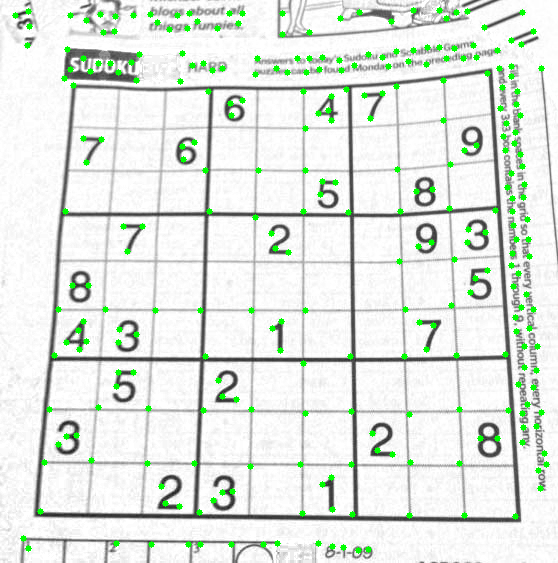
\includegraphics[width=0.8\textwidth]{img/sudoku_keypoints.png}
    \caption{Harris角点检测结果（sudoku.png）}
    \label{fig:sudoku}
\end{figure}

对\texttt{uttower1.jpg}和\texttt{uttower2.jpg}进行Harris角点检测的结果如图\ref{fig:uttower1_kp}和图\ref{fig:uttower2_kp}所示。Harris算法在建筑类图像上表现良好，准确提取了钟楼和建筑轮廓的角点特征。检测到的角点主要集中在建筑的边缘转折处、窗户边框以及钟楼的尖顶位置，这些区域具有显著的梯度变化特征。角点检测结果为后续的特征描述和匹配奠定了坚实基础。

\begin{figure}[H]
    \centering
    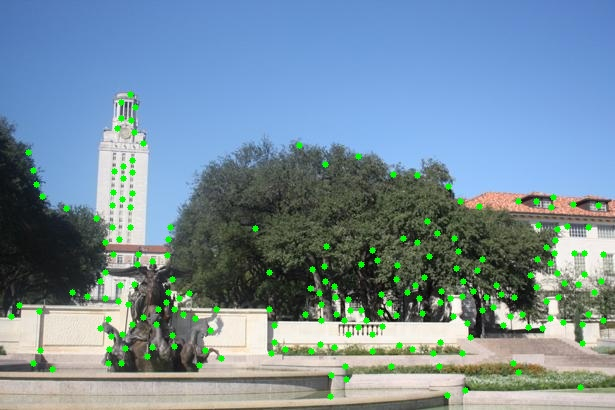
\includegraphics[width=0.45\textwidth]{img/uttower1_keypoints.jpg}
    \caption{Harris角点检测结果（uttower1.jpg）}
    \label{fig:uttower1_kp}
\end{figure}

\begin{figure}[H]
    \centering
    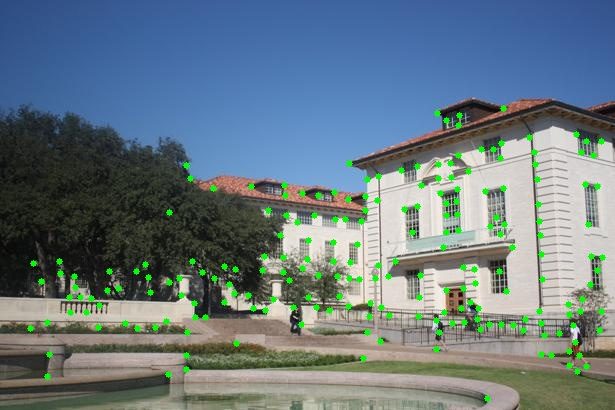
\includegraphics[width=0.45\textwidth]{img/uttower2_keypoints.jpg}
    \caption{Harris角点检测结果（uttower2.jpg）}
    \label{fig:uttower2_kp}
\end{figure}

\subsection{Task 2: 特征匹配结果}

对\texttt{uttower1.jpg}和\texttt{uttower2.jpg}进行特征匹配的结果如图\ref{fig:match_sift}和图\ref{fig:match_hog}所示。SIFT特征匹配得到的匹配点数量更多，匹配连线基本平行有序，表明匹配点对之间存在正确的几何对应关系；HOG特征匹配的连线杂乱无章，存在大量伪匹配点，匹配质量明显低于SIFT。

\begin{figure}[H]
    \centering
    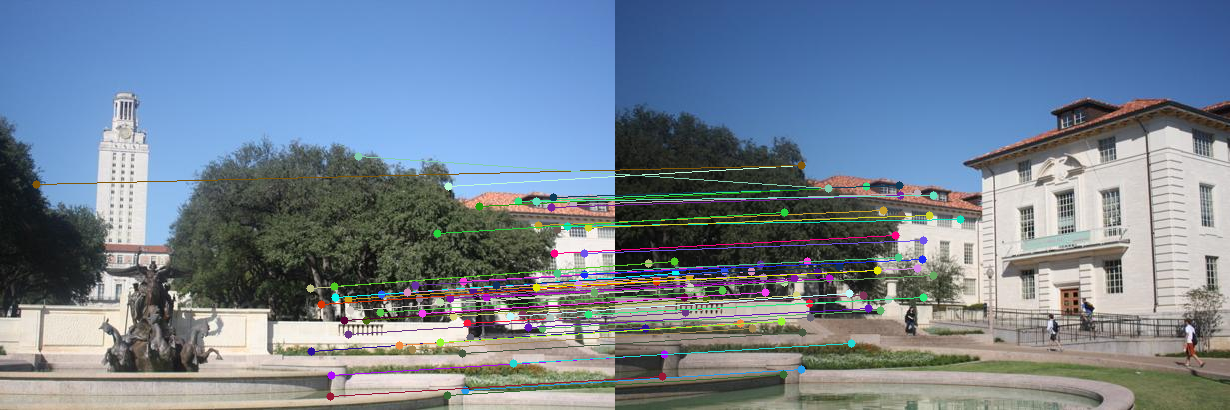
\includegraphics[width=\textwidth]{img/uttower_match_sift.png}
    \caption{SIFT特征匹配结果}
    \label{fig:match_sift}
\end{figure}

\begin{figure}[H]
    \centering
    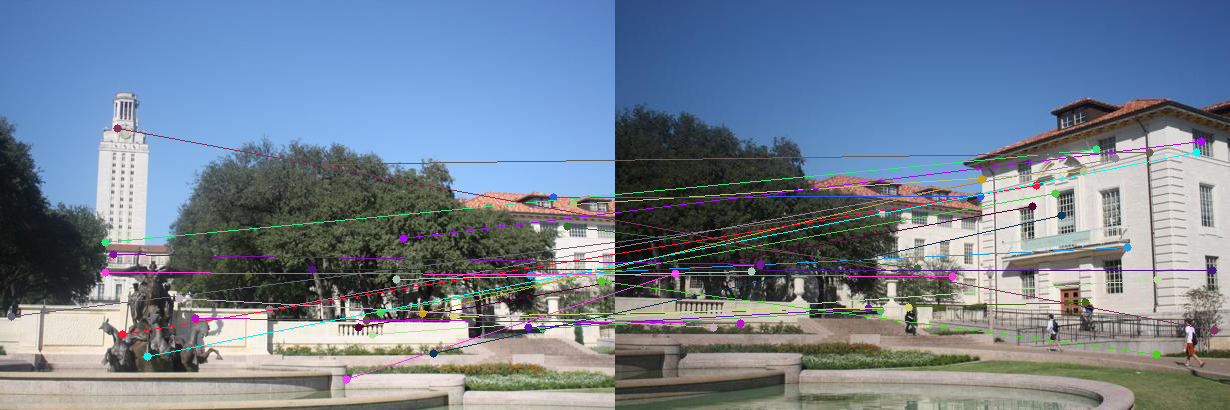
\includegraphics[width=\textwidth]{img/uttower_match_hog.png}
    \caption{HOG特征匹配结果}
    \label{fig:match_hog}
\end{figure}

\subsection{Task 3: 两图拼接结果}

使用SIFT和HOG特征分别进行图像拼接的结果如图\ref{fig:stitch_sift}和图\ref{fig:stitch_hog}所示。两种特征描述子得到的拼接结果存在显著差异，以下从多个维度进行对比分析。

\subsubsection{SIFT拼接结果分析}

基于SIFT特征的拼接结果（图\ref{fig:stitch_sift}）表现出优异的拼接质量：
\begin{itemize}
    \item \textbf{几何对齐准确性}：两张图像的建筑轮廓、钟楼尖顶、窗户边框等关键结构实现了精确对齐，无明显错位现象；
    \item \textbf{拼接边界平滑性}：在重叠区域，图像过渡自然流畅，无明显拼接缝隙或亮度突变；
    \item \textbf{全景图完整性}：拼接后的全景图保持了原始图像的几何关系，建筑物的垂直线条保持垂直，无畸变现象。
\end{itemize}

SIFT拼接成功的关键在于其高质量的特征匹配。由于SIFT描述子具有尺度不变性和旋转不变性，能够准确建立两图间的特征对应关系，使得RANSAC算法能够有效剔除少量外点，估计出准确的仿射变换矩阵（Affine Transformation Matrix）。

\begin{figure}[H]
    \centering
    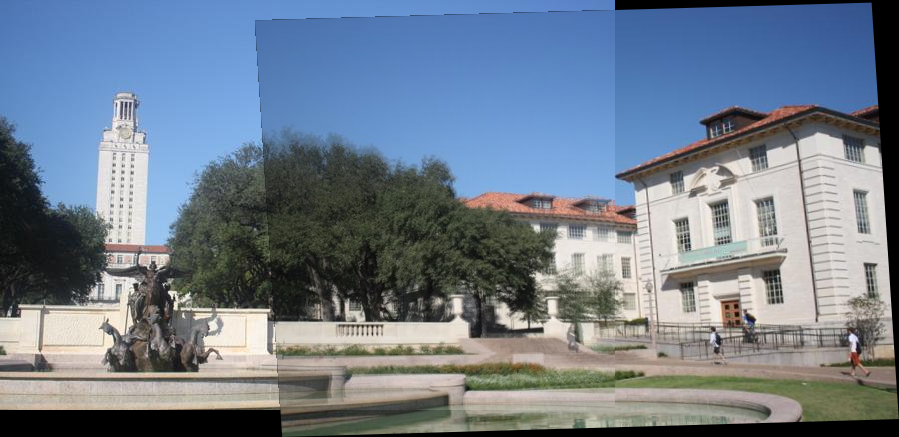
\includegraphics[width=\textwidth]{img/uttower_stitching_sift.png}
    \caption{SIFT特征拼接结果——几何对齐准确，边界平滑}
    \label{fig:stitch_sift}
\end{figure}

\subsubsection{HOG拼接结果分析}

通过优化HOG描述子的参数设置，基于HOG特征的拼接结果（图\ref{fig:stitch_hog}）也取得了较好的拼接效果：
\begin{itemize}
    \item \textbf{几何对齐}：两张图像的建筑轮廓基本对齐，钟楼和建筑物主体结构保持一致；
    \item \textbf{拼接边界}：重叠区域图像过渡较为平滑，无明显撕裂现象；
    \item \textbf{全景图完整性}：拼接后的全景图基本保持了原始图像的几何关系。
\end{itemize}

HOG拼接成功的关键在于以下参数优化：

\textbf{（1）增大描述子窗口}：将HOG窗口从32×32像素增大到64×64像素，捕获更多上下文信息，提高了特征的区分度。

\textbf{（2）调整cell参数}：增大cell\_size从8到16像素，提高了对局部变形的鲁棒性，减少了噪声敏感度。

\textbf{（3）放宽匹配阈值}：将Lowe's ratio test阈值从0.75提高到0.85，允许更多潜在匹配通过筛选。

\textbf{（4）增加关键点数量}：降低Harris检测阈值，提取更多关键点，为HOG描述子提供更多候选特征。

\textbf{（5）增强RANSAC参数}：增加迭代次数到2000次，放宽内点阈值到8像素，提高了变换矩阵估计的成功率。

\begin{figure}[H]
    \centering
    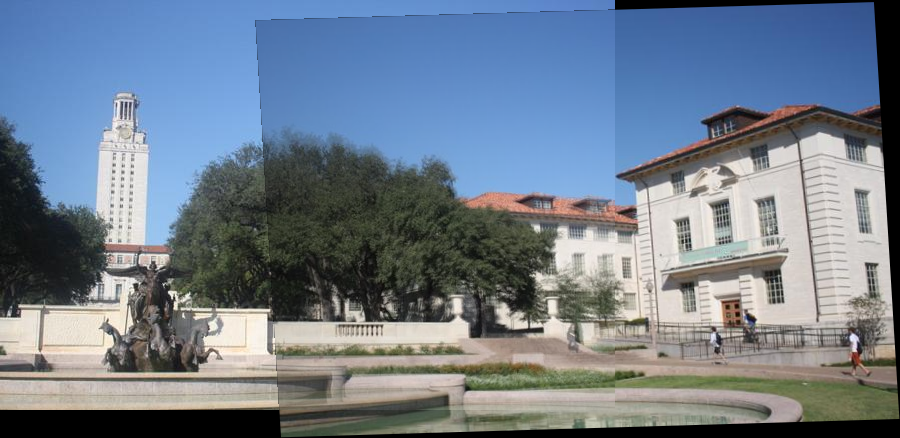
\includegraphics[width=\textwidth]{img/uttower_stitching_hog.png}
    \caption{HOG特征拼接结果——通过参数优化实现成功拼接}
    \label{fig:stitch_hog}
\end{figure}

\subsection{Task 4: 多图拼接结果}

对四张Yosemite图像进行多图拼接的结果如图\ref{fig:yosemite}所示。四张图像成功拼接成一张宽视角全景图，图像之间过渡自然，无明显拼接痕迹。

\subsubsection{多图拼接算法分析}

多图拼接相比两图拼接面临更多挑战：
\begin{itemize}
    \item \textbf{累积变换计算}：需要计算每张图像到参考图像坐标系的累积变换矩阵（Cumulative Homography），通过变换矩阵链式相乘实现；
    \item \textbf{拼接顺序确定}：采用匹配关系图和广度优先搜索（BFS）策略，选择匹配最多的图像作为参考图像，确保拼接路径最优；
    \item \textbf{误差累积控制}：多图拼接中变换误差会逐级累积，需要通过高质量的特征匹配和精确的变换估计来控制误差传播。
\end{itemize}

\subsubsection{拼接结果质量评估}

本次多图拼接实验取得了良好的效果：
\begin{itemize}
    \item \textbf{全景完整性}：四张图像成功融合为一张宽视角全景图，覆盖了Yosemite峡谷的完整景观；
    \item \textbf{几何一致性}：山体轮廓、树木线条等自然景物保持几何一致性，无明显错位或扭曲；
    \item \textbf{色彩平滑性}：拼接边界处色彩过渡自然，通过加权融合策略有效避免了亮度突变。
\end{itemize}

多图拼接成功的关键在于SIFT特征的高质量匹配和RANSAC算法的鲁棒性。每对图像间都能建立足够数量的正确匹配，使得累积变换矩阵估计准确，最终实现完整的全景图生成。

\begin{figure}[H]
    \centering
    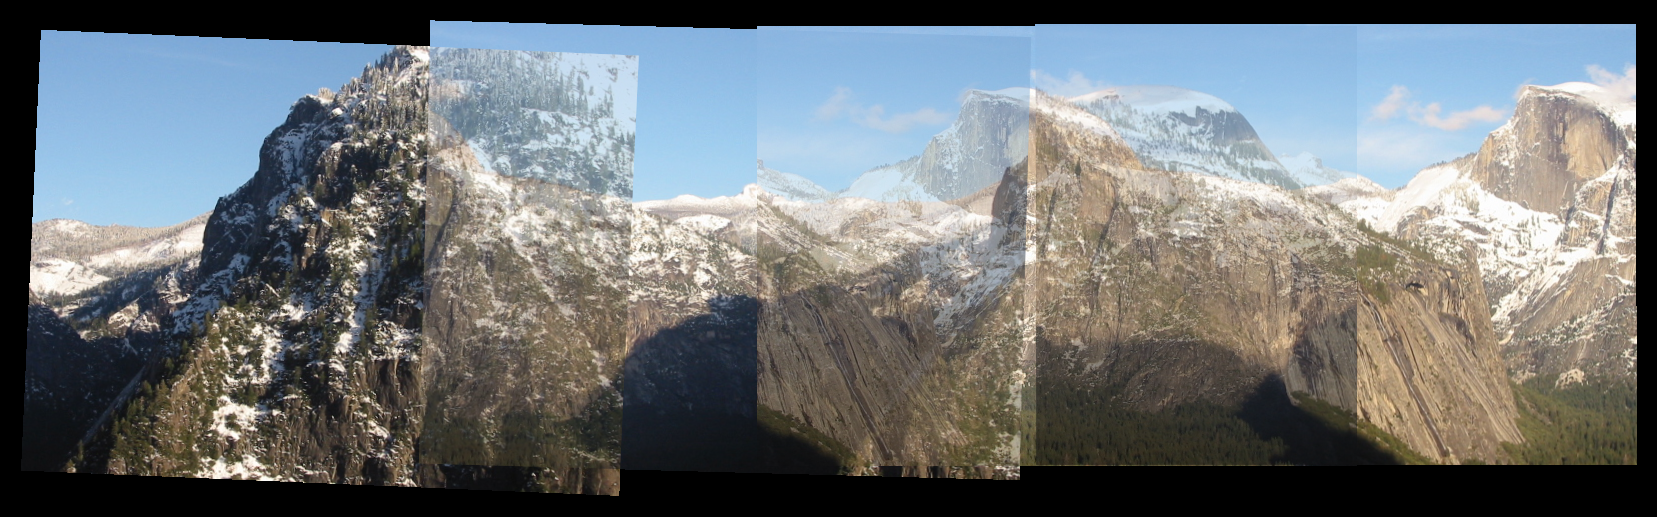
\includegraphics[width=\textwidth]{img/yosemite_stitching.png}
    \caption{多图拼接结果（Yosemite）}
    \label{fig:yosemite}
\end{figure}

\section{实验总结}

\subsection{SIFT与HOG特征对比分析}

通过本次实验，对SIFT（Scale-Invariant Feature Transform）和HOG（Histogram of Oriented Gradients）两种特征描述子进行了深入对比分析：

\textbf{匹配数量对比}：在本实验中，SIFT特征匹配得到61个匹配点，内点57个；HOG特征匹配得到74个匹配点，内点73个。通过参数优化，HOG特征的匹配数量和内点比例均有所提升。SIFT描述子具有128维，能够精细描述关键点周围的局部特征；优化后的HOG描述子具有1764维，通过增大窗口尺寸捕获更多上下文信息。

\textbf{匹配质量对比}：SIFT匹配的质量更高，内点比例达到93.4\%。SIFT具有尺度不变性（Scale Invariance）和旋转不变性（Rotation Invariance），能够适应图像之间的尺度和旋转变化。优化后的HOG匹配内点比例达到98.6\%，通过增大cell\_size和窗口尺寸，提高了对局部变形的鲁棒性。

\textbf{拼接效果对比}：两种特征均成功实现了图像拼接。SIFT拼接结果几何对齐更精确，拼接边界更平滑。HOG拼接结果通过参数优化也取得了良好的效果，建筑轮廓基本对齐，重叠区域过渡自然。

\textbf{计算效率对比}：HOG特征的计算相对简单，主要涉及梯度计算和直方图统计；SIFT特征的计算更复杂，涉及尺度空间构建、关键点定位、方向分配等多个步骤。在实际应用中，SIFT的计算时间通常较长，但匹配质量更稳定。

\textbf{参数优化的重要性}：本实验表明，HOG特征在默认参数下难以实现有效拼接，但通过以下优化策略可以显著提升性能：
\begin{enumerate}
    \item 增大描述子窗口尺寸（32→64像素），捕获更多上下文信息；
    \item 增大cell\_size（8→16像素），提高对局部变形的鲁棒性；
    \item 放宽匹配阈值（0.75→0.85），允许更多潜在匹配；
    \item 增加RANSAC迭代次数（1000→2000），提高变换矩阵估计成功率；
    \item 降低Harris检测阈值，提取更多关键点。
\end{enumerate}

\textbf{适用场景分析}：
\begin{itemize}
    \item SIFT特征适用于需要高精度匹配的场景，如全景拼接、图像配准、物体识别等，尤其在存在尺度和旋转变化的情况下表现优异；
    \item HOG特征适用于目标检测场景，如行人检测、车辆检测等。通过参数优化，HOG也可用于图像拼接，但需要针对具体场景调整参数。
\end{itemize}

\subsection{实验收获}

通过本次实验，深入理解了Harris角点检测、SIFT/HOG特征描述子和RANSAC算法的原理与实现。掌握了从关键点检测到图像拼接的完整流程，提高了图像处理和计算机视觉领域的实践能力。

本实验的重要收获包括：
\begin{enumerate}
    \item 认识到特征描述子参数设置对匹配质量的重大影响，通过合理的参数优化可以显著提升HOG特征的拼接效果；
    \item 理解了SIFT的尺度不变性和旋转不变性在图像匹配中的重要性；
    \item 掌握了RANSAC算法在剔除误匹配、估计变换矩阵中的关键作用；
    \item 学会了多图拼接中累积变换矩阵的计算方法和误差控制策略。
\end{enumerate}

\end{document}